\documentclass[review]{elsarticle}
\usepackage{lineno,hyperref}
\modulolinenumbers[5]
\usepackage[margin=1in]{geometry}
\usepackage{graphicx}
\usepackage{amsmath}
\usepackage{placeins}
\usepackage{comment}
\usepackage{gensymb}
\usepackage{flexisym}
\usepackage{color}
\usepackage[title]{appendix}

\journal{Journal of Nuclear Materials}
\bibliographystyle{elsarticle-num}

\begin{document}

\begin{frontmatter}
\title{Determination of thermal expansion, defect formation energy, and defect-induced strain of $\alpha$-U via \textit{ab initio} molecular dynamics}

\author[ncsu,inl]{Benjamin Beeler\corref{qwe}}
\cortext[qwe]{Corresponding author}
\ead{bwbeeler@ncsu.edu}
\author[ncsu]{Khadija Mahbuba}
\author[mich]{Yuhao Wang}
\author[inl]{Andrea Jokisaari}
\address[ncsu]{North Carolina State University, Raleigh, NC 27607}
\address[inl]{Idaho National Laboratory, Idaho Falls, ID 83415}
\address[mich]{University of Michigan, Ann Arbor, MI 48109}

\begin{abstract}

Uranium (U) is often alloyed with molybdenum (Mo) or zirconium (Zr) in order to stabilize its high-temperature body-centered cubic phase for use in nuclear reactors. However, in all metallic fuel forms, the $\alpha$ phase of U remains in some fraction. This phase decomposition due to temperature or compositional variance can play an outsized role on fuel performance and microstructural evolution. Relatively little is known about fundamental point defect properties in $\alpha$-U at non-zero temperatures, from either computational or experimental studies. This work performs the first thorough evaluation of the $\alpha$ phase of U via \textit{ab initio} molecular dynamics (AIMD). A number of thermophysical properties are calculated as a function of temperature, including equilibrium lattice parameters, thermal expansion, bulk modulus, and heat capacity. These results indicate a two-region behavior, with the transition at 400 K. The thermal expansion expansion/contraction in the \textit{a}/\textit{b} direction occurs rapidly from 100 K up to 400 K, after which a more linear and gradual change in the lattice constant takes place. The volumetric expansion matches experiments quantitatively, but the individual lattice constant expansion only matches experiments qualitatively. Point defect formation energies and induced lattice strains are also determined as a function of temperature, providing insight on defect populations and the fundamentals of irradiation growth in $\alpha$-U. Interstitials induce significantly more strain than vacancies, and the nature of that strain is highly dependent on the individual lattice directions. The direction of point defect induced lattice strain is contrary to the irradiation growth behavior of $\alpha$-U. This work shows that isolated point defects cannot be the primary driving force responsible for the significant irradiation induced growth of $\alpha$-U observed experimentally. 

\end{abstract}
\end{frontmatter}

\section{Introduction}

Uranium (U) is an actinide element exhibiting delocalized f-electrons that exists in three solid phases: $\alpha$ (face-centered orthorhombic), $\beta$ (tetragonal with a 30 atom unit cell) and $\gamma$ (body-centered cubic) \cite{yoo1998}. Below 935 K, U exists in the $\alpha$ phase \cite{soderlind1998}. Although uranium is alloyed with Mo or Zr in order to stabilize the preferred body-centered cubic phase at lower temperatures, most notably for nuclear fuel applications, the $\alpha$ phase persists either in decomposed phase regions (as in the case of U-Mo fuel), or in the low temperature periphery of the fuel slug (as in the case of U-Zr type fuel). Because of its unique crystal structure, $\alpha$-U exhibits anisotropic material properties, for example, thermal expansion \cite{lloyd1966} and elastic constants \cite{fisher1958}. One relevant behavior is the anistropic irradiation growth of $\alpha$-U \cite{leggett1963}, which can lead to the formation of crystallographically aligned pores ($\alpha$-tearing). These pores are believed to form due to the interaction of lattice defects and stresses induced by irradiation and a temperature gradient, and result in significant volume changes of $\alpha$-U \cite{leggett1963,paine1958}. A full understanding of the relationship between point defects, lattice strains, and the generation of pores, has not been established either experimentally or via computational methods. However, a number of computational studies have been performed into fundamental properties of uranium. 

Density functional theory (DFT) is an essential part of computational materials science, addressing a variety of problems in materials design and processing on a fundamental level. Several examinations of U via DFT have been performed on its orthorhombic and body-centered cubic (bcc) structures. Taylor \cite{taylor2008} used a projector augmented wave (PAW) pseudopotential to calculate the lattice constants of $\alpha$-U and $\gamma$-U along with the bulk modulus of both phases and the surface energy of a single surface in $\alpha$-U. Xiang, \textit{et al.} \cite{xiang2008} also utilized a PAW pseudopotential to perform an analysis of lattice constants in the $\alpha$ and $\gamma$ phases, as well as an analysis of defects in $\gamma$-U. Beeler, \textit{et al.} calculated the lattice constants and elastic constants of $\alpha$, $\beta$ and $\gamma$-U \cite{beeler2013}, in addition to the point defect properties in both $\alpha$ and $\gamma$-U \cite{beeler2010}. Huang and Wirth \cite{wirth2011, wirth2012} calculated intrinsic and extrinsic point defect formation energies and migration barriers in $\alpha$-U. These DFT investigations showed a general, if imperfect, agreement with the experimental bulk moduli, lattice and elastic constants, and vacancy formation energy \cite{yoo1998, barrett1963, matter1980}. 

Key areas lacking from the DFT-based literature on $\alpha$-U include an analysis of temperature-dependent bulk properties, including thermal expansion and heat capacity, and temperature-dependent defect properties. Extrapolation of 0 K properties to compare to elevated temperature experiments can be ill-advised, particularly for complex crystal structures or for point defects. However, \textit{ab initio} molecular dynamics (AIMD) allows for quantum mechanical-based calculations to be performed at non-zero temperatures. AIMD has been utilized to study a variety of systems including liquid phase diffusion in Al-Si \cite{manga2018}, adsorption energy of Fe on TiN surfaces \cite{wang2010}, NaCl dissolution in water \cite{timko2010} and finite temperature phonon dispersion curves in bcc Zr and bcc Li \cite{hellman2011}. Hood, \textit{et al.} \cite{hood2008} have previously utilized AIMD to study the equation of state of U and the variation in density of states for the liquid phase of U at two unique temperatures. Hood, \textit{et al.} utilized a unique pseudopotential that was presented in that same manuscript \cite{hood2008}. Soderlind, \textit{et al.} \cite{soderlind2012} utilized self-consistent \textit{ab initio} lattice dynamics (SCAILD) to study the high temperature stabilization of the $\gamma$-U phase by calculating phonon modes at 1100 K. There have been several investigations of the free energy via the temperature dependent effective potential (TDEP) technique \cite{hellman2013, ladygin2020, kruglov2019, bouchet2017, castellano2020}, and one recent AIMD investigation into the defect formation energies in $\gamma$-U at high temperatures \cite{beelerAIMD}. Despite numerous investigated into metallic uranium, AIMD has not been deployed to study temperature dependent properties of $\alpha$-U, such as thermal expansion or defect formation energies. 

In this work, AIMD simulations are performed to calculate the equilibrium volume of $\alpha$-U as a function of temperature. Utilizing these equilibrium volumes, the three lattice constants of $\alpha$-U are determined, yielding anisotropic thermal expansion calculations. Additionally, point defect formation energies for interstitials and vacancies are calculated as a function of temperature. The lattice strain from the introduction of these point defects is calculated, providing insight into the fundamental stages of irradiation growth. Finally, surface energies of $\alpha$-U are calculated for a select number of surfaces, allowing for comparison to previous computational studies and integration into mesoscale fuel performance models. This is the first AIMD investigation of point defects in $\alpha$-U. 

\section{Computational Details}
Systems are investigated using the Vienna \textit{ab initio} Simulation Package (VASP) \cite{vasp1, vasp2, vasp3, vasp4}. The projector augmented wave (PAW) method \cite{paw1, paw2} is utilized within the density functional theory \cite{dft1, dft2} framework. Calculations are performed using the Perdew-Burke-Ernzerhof (PBE) \cite{pbe1, pbe2} generalized gradient approximation (GGA) density functional implementation for the description of the exchange-correlation. A uranium PAW pseudopotential with the 6s$^{2}$6p$^{6}$5f$^{3}$6d$^{1}$7s$^{2}$ valence electronic configuration and a core represented by [Xe, 5d, 4f] is utilized. Methfessel and Paxton's smearing method \cite{methfessel} of the first order is used with a width of 0.1 eV to determine the partial occupancies for each wavefunction. A Monkhorst-Pack \cite{monkhorst} 1x1x1 k-point mesh was utilized for Brillouin zone sampling. Uranium is assumed to be non-magnetic, in accordance with both experiments \cite{chembook} and previous simulations \cite{beeler2013}, and as such calculations are non-spin-polarized. The Hubbard U term is not applied to the \textit{f} electrons, in accordance with previous computational studies that utilized DFT on $\alpha$-U \cite{wirth2011, wirth2012, taylor2008, beeler2013}. The precision is set to normal and the energy cutoff is increased to 300 eV. The electronic self-consistent loop exit criterion is set to 10$^{-4}$ and the precision for projectors in real space is increased to -10$^{-4}$. A 180 atom supercell (5x3x3 unit cells) is utilized for all simulations. Such a supercell is sufficiently large to preclude defect-defect interactions. Dynamics were carried out in the NpT ensemble with Parinello-Rahman dynamics and a Langevin thermostat to control temperature. The temperature range investigated is from 100 K to 800 K, in increments of 100 K, to span nearly the entire range of stability of the $\alpha$ phase of U. The Langevin friction coefficient for both the atomic and lattice degrees-of-freedom was set to 5 ps$^{-1}$, with a fictitious mass for the lattice degrees of freedom of 500 amu. The timestep is set to 2.0 fs, and the initial structures are equilibrated at the target temperature for 8 ps. The trajectories of the total supercell energy, pressure, and individual lattice vectors are analyzed as a function of timestep to ensure that an equilibrated state has been reached and each of these quantities are oscillating around a given value, with the pressure oscillating around zero. Subsequently, the simulations are further equilibrated for 2000 timesteps (4 ps) for the determination of equilibrium properties. In order to obtain average properties over the \textit{ab initio} molecular dynamics simulation, the energies and lattice constants for the final 1500 timesteps (3 ps) are extracted and averaged. In order to ensure statistical significance of the results, ten unique simulations are performed for each individual simulation setup. 

The thermal expansion is calculated both for individual lattice constants, and as a volume averaged value, via equation \ref{eq:exp}:

\begin{equation}
\label{eq:exp}
\alpha = \frac{L-L_0}{L_0} 
\end{equation}

where $\alpha$ is the thermal expansion, and L is the length of the individual lattice constant (or averaged lattice constant) at a given temperature, and L$_0$ is the reference length at a given temperature. The formation energy of point defects is calculated via equation \ref{eq:eform}: 

\begin{equation}
\label{eq:eform}
E_f = E^* - \frac{n \pm 1}{n} \times E_0
\end{equation}

where E$^{*}$ is the energy of a system with a defect (with n $\pm 1$ atoms), \textit{n} is the number of atoms in the defect-free system and E$_{0}$ is the energy of a defect-free system with \textit{n} atoms. Equation \ref{eq:eform} utilizes (\textit{n} + 1) for interstitials and (\textit{n} - 1) for vacancies. The molar heat capacity is determined from equation \ref{eq:cp}:

\begin{equation}
\label{eq:cp}
C_{P} = \left(\frac{\delta H}{\delta T}\right)_{P}
\end{equation}

where H is the enthalpy (potential plus kinetic energy), T is the temperature, and it is emphasized that this is determined for a constant pressure, which in these simulation is zero pressure. The total heat capacity is a sum of the lattice (Eq. \ref{eq:cp}) and the electronic components of the heat capacity. The electronic heat capacity coefficient ($\gamma_e$, where the electronic heat capacity is $\gamma_e\times$T) has been experimentally reported \cite{marchidan1976, schachinger1989} to be 10.12 mJ/mol-K$^2$, and this value is utilized here to determine the total heat capacity as a function of temperature. 

\begin{comment}
Surfaces are generated by constructing a crystal structure with an adjacent section of vacuum, within a periodic boundary supercell. This simulation setup generates two identical surfaces within a single supercell. Five unique surface orientations are included in the analysis: (1 0 0), (0 1 0), (0 0 1), (3 2 0), and (0 36 $\bar{25}$). Due to the anisotropy of the crystal structure, each of the primary planes presents a unique surface, and the two off-primary planes are chosen because they have previously been shown to be of interest in $\alpha$-U \cite{khadija1}. Supercells must be generated to size both parallel and perpendicular to the interface to ensure that the appropriate crystal structure is remaining stable and that surfaces are non-interacting. Convergence examinations were performed that showed a requirement of minimum surface-parallel dimensions of approximately 1-1.5 nm, and surface-perpendicular dimensions of approximately 3 nm (with approximately 1 nm of vacuum). This results in supercell sizes on the order of 250 to 300 atoms. The surface energies are determined from equation \ref{eq:surf}:

\begin{equation}
\label{eq:surf}
E_f^{surf} = \frac{E^* - N\times E_{at}}{2A} 
\end{equation}

where E$^*$ is the energy of a system with two surfaces, E$_{at}$ is the energy per atom of the pure crystalline system, and A is the surface area of a single surface. 

\end{comment}

\section{Results}
\subsection{Equilibrium properties of $\alpha$-U}

The equilibrium lattice constants at room temperature were calculated to be: \textit{a} = 2.78 \AA, \textit{b} = 5.91 \AA, and \textit{c} = 4.93 \AA. These results compare very favorably to the experimental literature (\textit{a} = 2.85\AA, \textit{b} = 5.86\AA, and \textit{c} = 4.96 \AA \cite{lawson1988}), with the largest deviation observed for the \textit{a} lattice constant at a magnitude of approximately 2.5\%. Some deviation is not unexpected, as it has been shown that DFT calculations do not always exactly match the experimental findings, particularly for the lattice constant. However, these results are in accordance with previously computational investigations of $\alpha$-U performed at 0 K, when thermal expansion is taken into account \cite{wirth2011,beeler2013}. 

The normalized lattice constants as a function of temperature are shown in Fig. \ref{fig:a0}. Each lattice constant is normalized to its determined value at 100 K, which is the lowest temperature analyzed. Thermal expansion occurs in both the \textit{a} and \textit{c} directions, while thermal contraction occurs in the \textit{b} direction, as has been previously experimentally observed \cite{grenthe2010}. Average values for linear thermal expansion coefficients of $\alpha$-U for the \textit{a}, \textit{b}, and \textit{c} crystallographic directions were experimentally determined to be 26.5$\times$10$^{-6}$ K$^{-1}$, -2.4$\times$10$^{-6}$ K$^{-1}$, and 23.9$\times$10$^{-6}$ K$^{-1}$, respectively, over temperature range of 298-598 K \cite{grenthe2010, lloyd1966}. The data in Fig. \ref{fig:exp} utilizes 300 K as the reference point for both the AIMD data and the experimental data, and as such, the change in length at 300 K is zero. It can be observed that the AIMD predicted thermal expansion in the \textit{a} direction is significantly greater than that determined from experiment. Similarly, the amount of contraction in the \textit{b} direction predicted from AIMD is significantly greater than that observed in experiments. However, the \textit{c} direction exactly matches the linear thermal expansion determined from experiments. Qualitatively, all of the behaviors are identical, with the \textit{a} and \textit{b} directions expressing a more extreme expansion/contraction behavior. The source of the deviations from experiment are currently unknown. It should be noted that significant scatter exists in the experimental datasets utilized to generate the averages presented for comparison in Fig. \ref{fig:exp}, and additional experimental investigations are warranted in order to confirm previous findings.

 \begin{figure}[hbt]
	\centering
	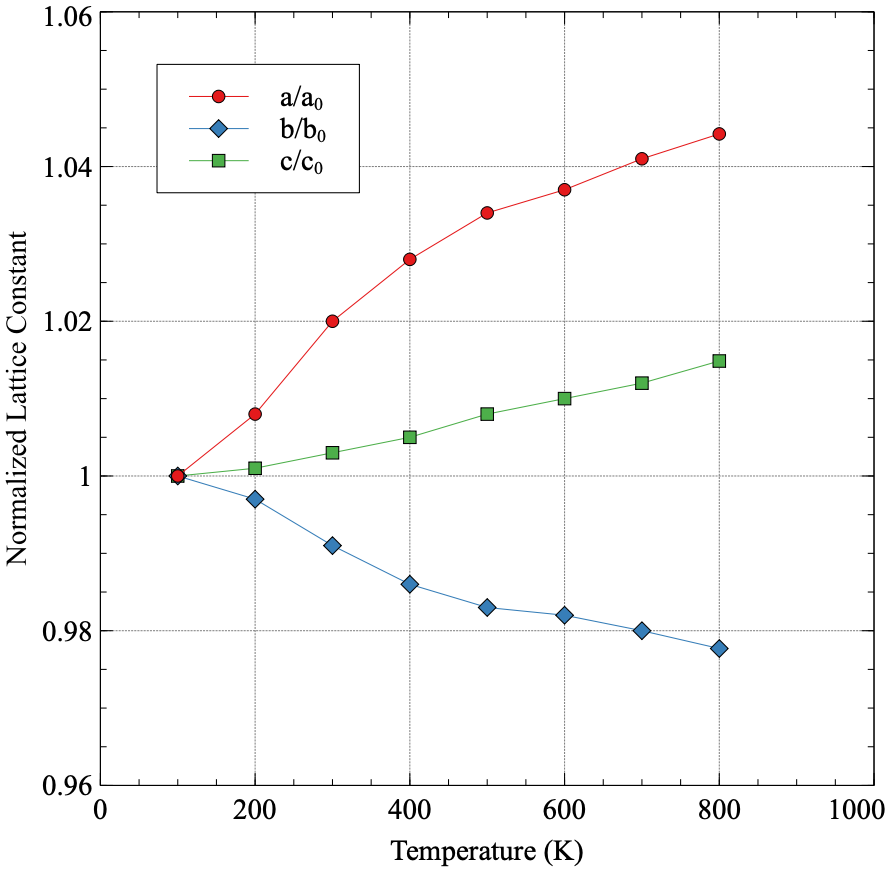
\includegraphics[width=0.6\textwidth]{fig1.png}
    \caption{The normalized lattice constants as a function of temperature for $\alpha$-U. Each lattice constant is normalized to its value at 100 K.}\label{fig:a0}
\end{figure}



 \begin{figure}[hbt]
	\centering
	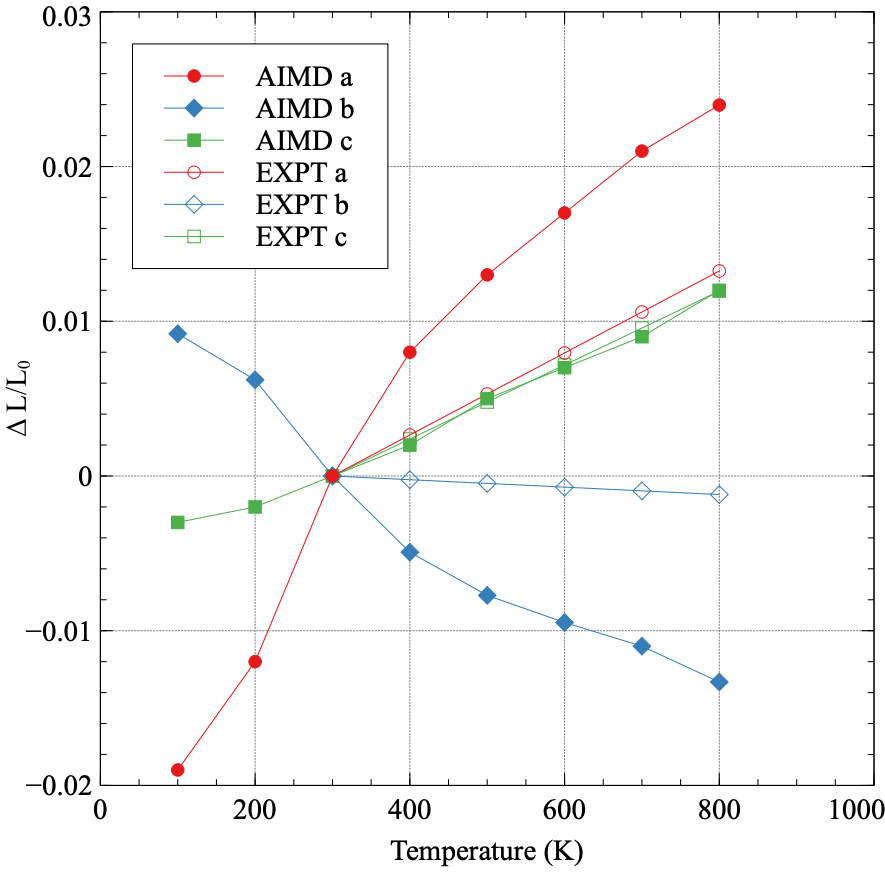
\includegraphics[width=0.6\textwidth]{fig2.png}
    \caption{The linear thermal expansion coefficient for each lattice constant in $\alpha$-U. Thermal expansion is normalized to 300 K, which is the lowest temperature in the experimental data \cite{grenthe2010, lloyd1966}. }\label{fig:exp}
\end{figure}

\FloatBarrier

The volume-averaged thermal expansion is calculated and compared to a different set of experimental results from Touloukian \cite{touloukian} in Fig. \ref{fig:vol}. Interestingly, the data from AIMD nearly exactly matches the experimental results for volumetric thermal expansion, with only slight deviations presenting above 600 K. Thus, despite the differences in the individual components of thermal expansion in $\alpha$-U, which are somewhat substantial, the cumulative effect on total volume expansion reproduces the experimental observations. 

 \begin{figure}[hbt]
	\centering
	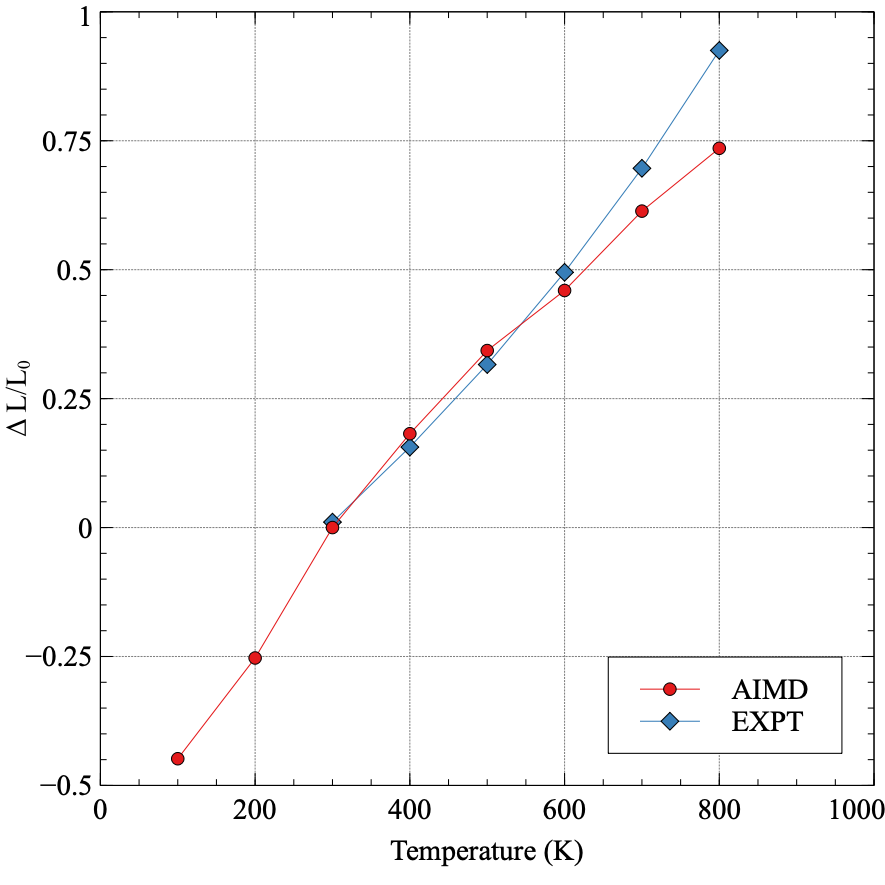
\includegraphics[width=0.6\textwidth]{fig3.png}
    \caption{Volume-averaged linear thermal expansion in $\alpha$-U. Thermal expansion is taken with respect to 300 K and compared to experimental results \cite{touloukian}.}\label{fig:vol}
\end{figure}

\FloatBarrier

The total constant pressure heat capacity is determined from a summation of equation \ref{eq:cp} and the electronic heat capacity contribution as determined by experiments, and plotted in Fig. \ref{fig:cp}. Temperatures shown are intermediate temperatures from those of study in this work, as the formalism in equation \ref{eq:cp} assumes effectively a constant value of C$_p$ over the temperature range. Thus, utilizing data points at 100 K and 200 K, for example, yields a value of C$_p$ at 150 K in this work. Experimental data is only reported for room temperature and upwards, and the agreement with the AIMD is generally excellent. The maximum deviation is observed at 750 K, where the AIMD results under-predict the magnitude of C$_p$ by approximately 11\%. At lower temperatures, the deviation can be less than 5\%. Thus, while the magnitude of the heat capacity is generally the same, it appears that the experimentally observed heat capacity is more sensitive to temperature, showing a total change from 250-750 K of 17 J/mol-K, while AIMD only predicts at increase of 11 J/mol-K over this temperature range. 

 \begin{figure}[hbt]
	\centering
	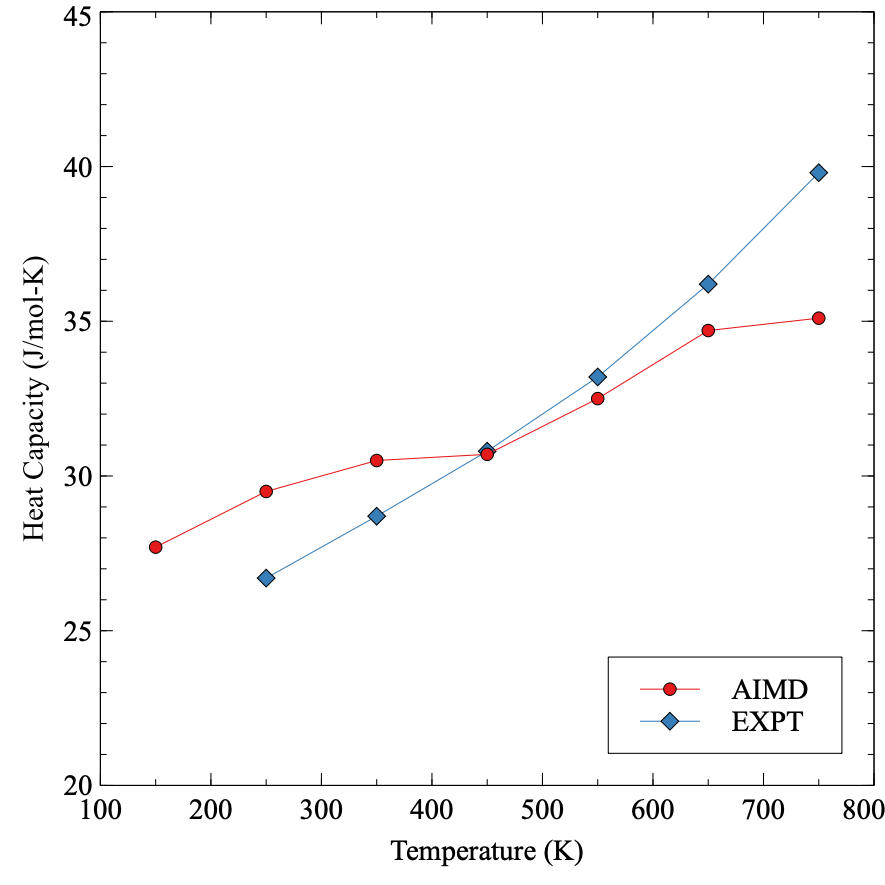
\includegraphics[width=0.6\textwidth]{fig_cp.png}
    \caption{The constant pressure heat capacity of $\alpha$-U from 100 K to 800 K. Results from this work are compared to experimental results from Konings \cite{konings2010}.}\label{fig:cp}
\end{figure}

\FloatBarrier

\begin{comment}
\begin{table}[h]
\caption{The constant pressure heat capacity of $\alpha$-U from 100 K to 800 K. Results from this work are compared to experimental results from Konings \cite{konings2010}. Units for heat capacity are in J/mol-K.} \label{tab:cp}
\begin{center}
\begin{tabular}{|c|c|c|}
	\hline
	Temperature (K) & AIMD & EXPT \\
	 \hline
	 150 & 27.7 & - \\
	 250 & 29.5 & 26.7 \\
	 350 & 30.5 & 28.7 \\
	 450 & 30.7 & 30.8 \\	 
	 550 & 32.5 & 33.2 \\
	 650 & 34.7 & 36.2 \\
	 750 & 35.1 & 39.8 \\
	 \hline
\end{tabular}
\end{center}
\label{default}
\end{table}
\end{comment}

\FloatBarrier

\subsection{Point defects in $\alpha$-U}

The point defect formation energy of interstitials and vacancies in $\alpha$-U is shown in Fig. \ref{fig:defs}. The defect formation energy for both types of defects tends to slightly decrease with increasing temperature, until approximately 400 K. Above 400 K, an increase in the defect formation energy with increasing temperature is observed. The relative magnitudes of the defect formation energies with respect to one another are near constant across the entire temperature range investigated, with the average interstitial formation energy (3.4 eV) about 2.3 times the average vacancy formation energy (1.46 eV). Error bars shown in Fig. \ref{fig:defs} are twice the standard error, where the standard error for formation energies is defined as 

\begin{equation}
\label{eq:surf}
SE^2 = \frac{\sigma_{bulk}}{\sqrt{N}} + \frac{\sigma_{def}}{\sqrt{N}}
\end{equation}

where $\sigma_{bulk/defect}$ is the standard deviation of the dataset utilized for determining the average energies of either the defect-free or the defected system, and \textit{N} is the sample size, which is ten simulations. The standard error in the data set tends to increase with increasing temperature, as would be expected. The results from the lower temperature regime can be compared to previous results from 0 K DFT calculation. At 100 K, the interstitial formation energy is found to be 3.81 eV, and the vacancy formation energy is found to be 1.69 eV. These results compare favorably to previous 0 K DFT results \cite{wirth2011}, which showed a vacancy formation energy of 1.69 eV (an exact match), and interstitial formation energy of 4.42 eV. That the interstitial formation energy from this work is lower is not unsurprising, as the effect of temperature can yield additional relaxation pathways or defect reorientation that is not strictly achievable through calculations at 0 K. However, the magnitude of the relaxation cannot be reasonably estimated from 0 K, and thus requires these high temperature calculations to determine true defect behavior at non-zero temperature. This data can be utilized to conduct higher length scale simulations which attempt to describe defect formation and mobility and those which include an estimation of the equilibrium concentrations of defects. 
 
 \begin{figure}[hbt]
	\centering
	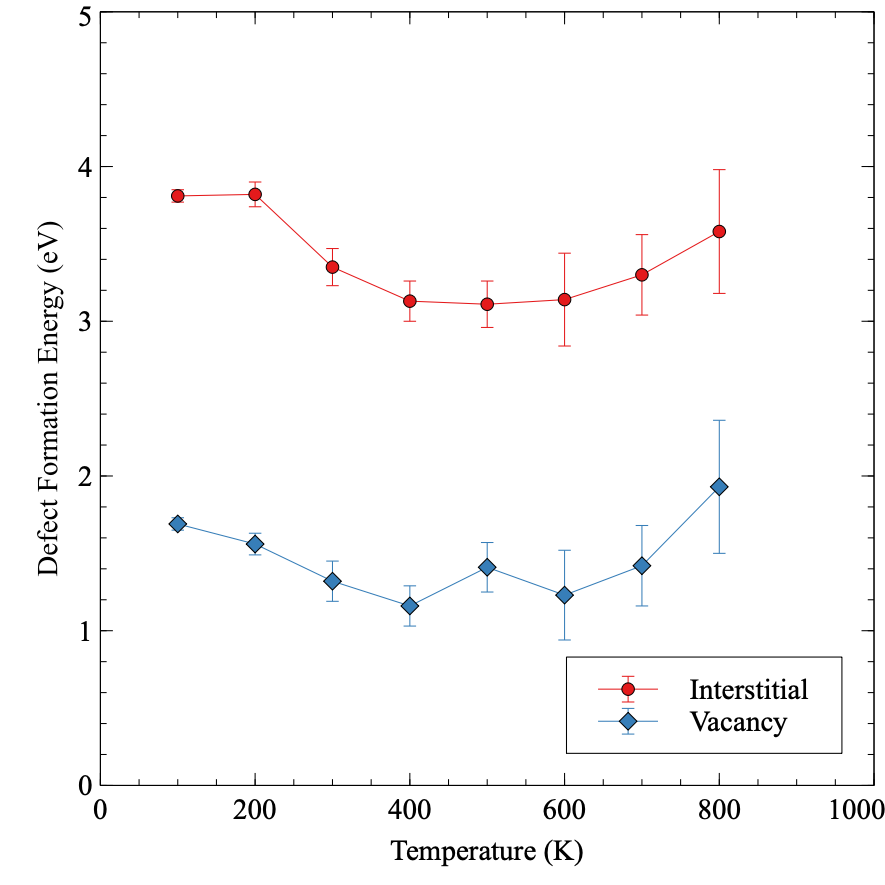
\includegraphics[width=0.6\textwidth]{fig4.png}
    \caption{The formation energy of an interstitial and a vacancy in $\alpha$-U as a function of temperature.}\label{fig:defs}
\end{figure}

\FloatBarrier

The introduction of a defect and relaxation in an NpT ensemble allows for the analysis of volume changes due to individual point defects. These volume changes are reported as a function of temperature in Fig. \ref{fig:strain}. For interstitials, there clearly exist two distinct regimes in the defect-induced strain environment, with 400 K serving as the demarcation temperature. Below 400 K, strain is relatively large and positive (lattice expansion) in the \textit{a} direction, and relatively large and negative (lattice compression) for the \textit{b} direction. The magnitudes of those strains decrease with increasing temperature up to 400 K, above which they maintain a relatively fixed value, with some statistical fluctuation. It is unknown whether the deviation at 600 K is due to some distinct behavioral changes, or is simply the result of thermal noise. However, data points at 600 K remains within the standard error of the general trend (standard error not shown here for readability of figures), which implies that it is unlikely to indicate a change in behavior. The \textit{c} lattice constant exhibits very slight positive strain across the entire temperature range, with no obvious changes in behavior. For vacancies, the general magnitude of the strain is significantly less than that observed for interstitials, with the maximum strain of 0.5\% observed at 800 K for the \textit{b} lattice constant. While it is more difficult to discern trends in the vacancy strain as a function of temperature, at several pieces of information can be readily extracted. The \textit{c} lattice constant displays no observed strain from vacancies at any temperature. For the \textit{a} and \textit{b} lattice constants, opposite trends present themselves above 400 K, in that the \textit{a} lattice constant strain increases with increasing temperature and the \textit{b} lattice constant strain decreases with increasing temperature. 

In a general sense, the strain behavior of defects is as expected, in that interstitials yield a lattice expansion, while vacancies produce lattice contraction. However, the manner in which those volumetric averages are produced is quite complex, and is significantly temperature dependent. 

 \begin{figure}[hbt]
	\centering
	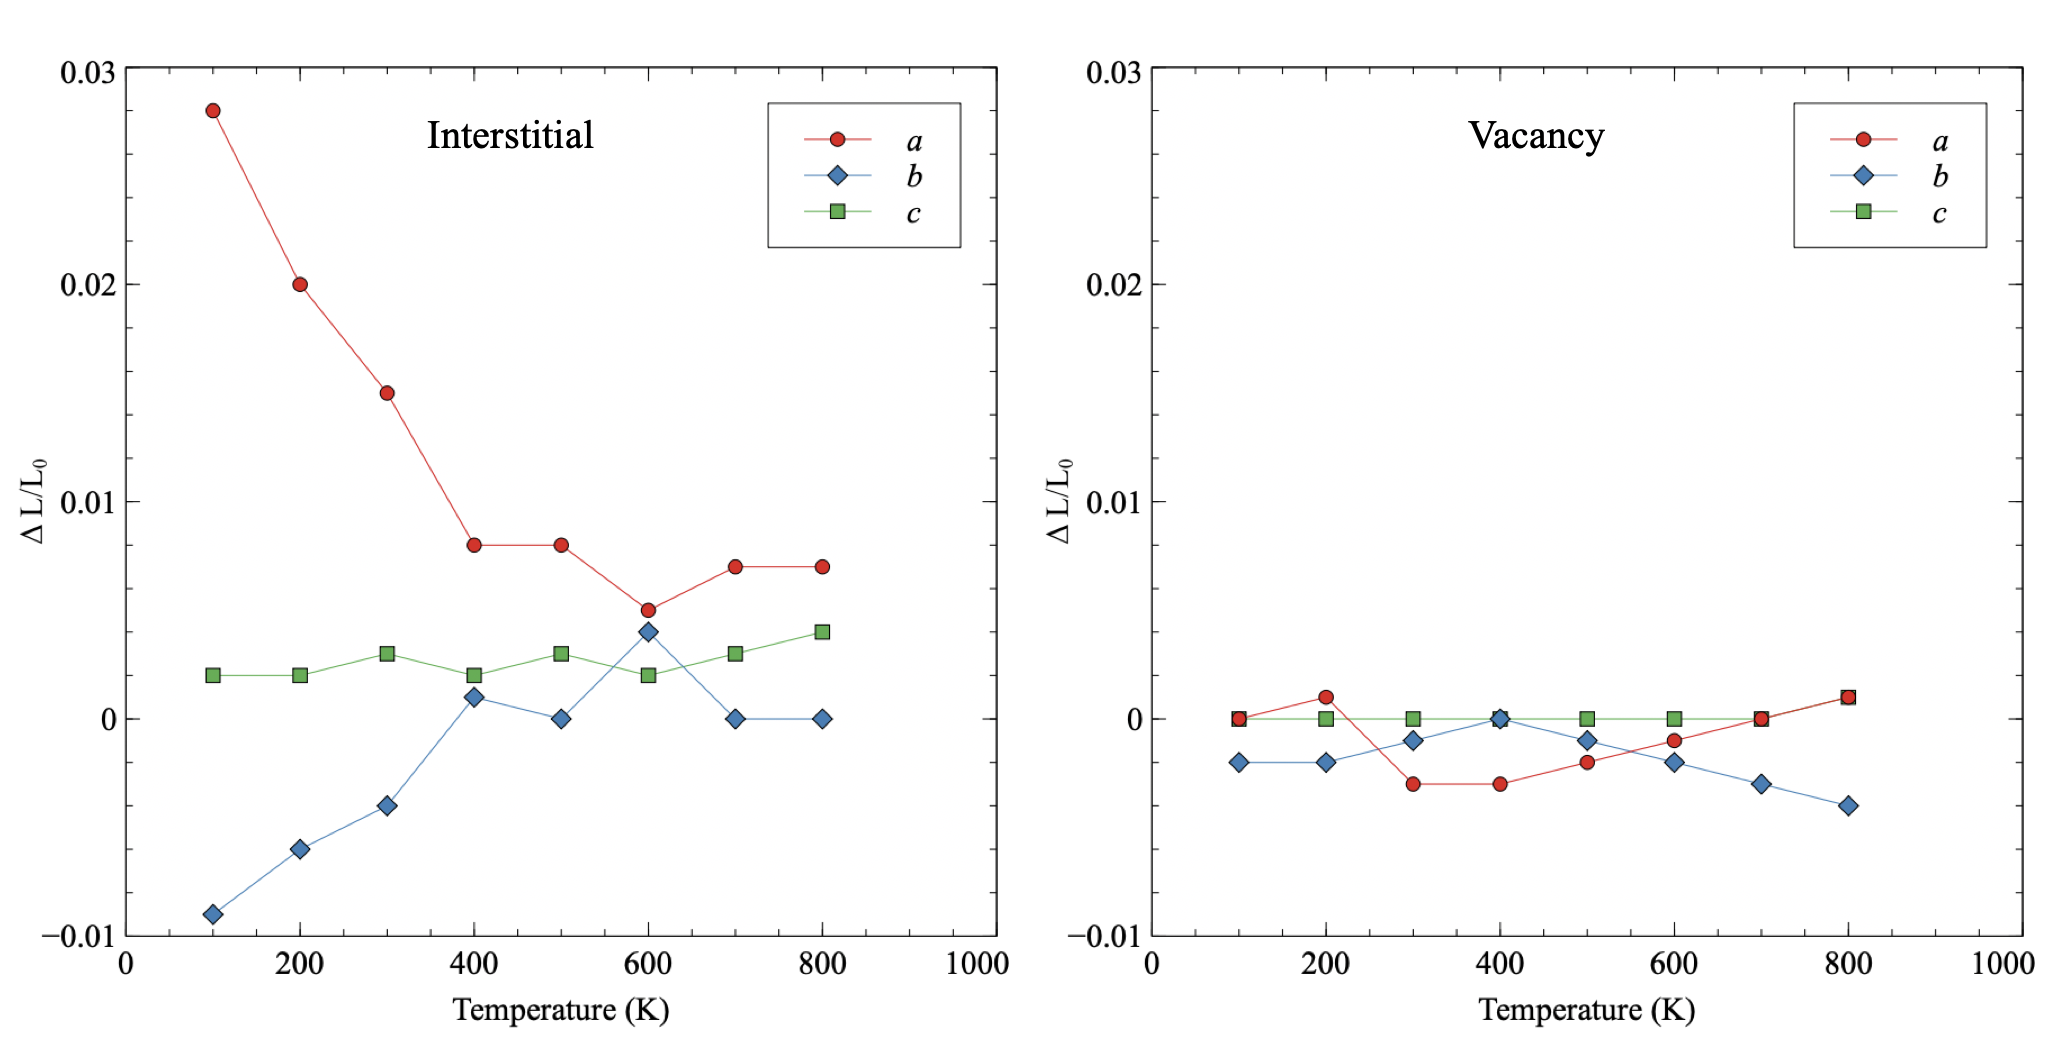
\includegraphics[width=1.0\textwidth]{fig5.png}
    \caption{The lattice strain induced from an interstitial or vacancy in $\alpha$-U as a function of temperature. }\label{fig:strain}
\end{figure}

\FloatBarrier

\section{Discussion}

This work indicates a number of lattice and volume effects that are strongly dependent upon the temperature of the system. Excepting the heat capacity, all of these calculated properties seem to indicate two regions of behavior, one below 400 K and one above 400 K. Also, it should be re-emphasized that the heat capacity utilized an experimental data point for the determination of the electronic heat capacity. Thus, from the purely computationally obtained data, there are differences in lattice constant, defect-induced lattice strain, and defect formation energy, in these two temperature regimes. To briefly summarize, thermal expansion expansion/contraction in the \textit{a}/\textit{b} direction occurs rapidly from 100 K up to 400 K, after which a more linear and gradual change in the lattice constant takes place. Defect formation energies decrease in magnitude up to 400 K, above which they tend to slightly increase. Defect lattice strains for interstitials decrease/increase in the \textit{a}/\textit{b} direction up to 400 K, above which they maintain essentially the same magnitude. A similar trend in defect lattice strains for vacancies is present, but the magnitude is significantly less and potentially swamped by thermal fluctuations, and thus the statistical certainty of the finding is reduced. 

In an attempt to identify underlying changes in the atomic and electronic structure as a function of temperature, two additional analyses were performed. The first of which was a coordination analysis, in which the radial distribution function (rdf) was constructed for a snapshot of the equilibrated $\alpha$-U structure at 200 K, 400 K, and 700 K. This coordination analysis yielded no discernible trend shifts, and the general bond length and peak broadening confirms what can already be observed in earlier figures in this manuscript outlining thermal expansion. The second analysis involved the electronic density of states (DOS). The electronic DOS as a function of temperature was calculated, and only minimal variation in the electronic structure was observed as a function of temperature. There was no indication that two regions of electronic structure behavior exist for the $\alpha$ phase. Due to the lack of identifiable structure variation as a function of temperature, these results are not displayed here, as the DOS and rdf can be obtained from the literature \cite{beeler2013,hood2008}. The underlying cause of the apparent two-region behavior is unclear, and warrants further computational investigation, in addition to experimental studies on high-purity uranium to either confirm or refute the findings in this work.

Comparison of the calculated direction of the defect-induced strains to the experimental literature on irradiation growth provides contradictory information. Paine and Kittel \cite{paine1958} and Loomis and Gerber \cite{loomis1968} both investigated dimensional change of single crystalline uranium under irradiation. Their findings were in general agreement with one another, and showed a contraction in the \textit{a} direction, an expansion in the \textit{b} direction, and no change in the \textit{c} direction. While the AIMD results presented here agree with the \textit{c} direction, exactly the opposite behavior is observed in Fig. \ref{fig:strain} for the \textit{a} and \textit{b} directions. This work showed interstitials as the dominant strain inducers, and expansion in the \textit{a} direction and contraction in the \textit{b} direction. It should be noted that this experimentally observed irradiation behavior is also in the opposite direction of the thermal expansion of the individual lattice constants. Given that isolated point defects lead to the opposite trends from those observed experimentally, it is possible that defect clusters or defect loops display different strain behaviors than individual point defects, and are more responsible for irradiation growth in $\alpha$-U. Such research is beyond the scope of AIMD, which is currently sufficiently computationally expensive to exclude the possibility of analysis of extended defects. Thus, classical molecular dynamics simulations can be performed, and validated against the work presented here. Ideally, in addition to further computational studies, the experimental results from over sixty years ago should be reproduced and modern characterization methods applied to extract fundamental defect populations, densities, and orientations. 

\section{Conclusions}

In this study, AIMD simulations were performed to calculate temperature-dependent properties of the $\alpha$ phase of U from 100 K to 800 K. The thermal expansion of each individual lattice constant was analyzed and compared to the experimental literature. Although the general direction of thermal expansion corresponded to the experimental findings (positive in \textit{a} and \textit{c}, negative in \textit{b}), the magnitudes of coefficient of thermal expansion for the \textit{a} and \textit{b} directions was greater than that observed experimentally. However, the volumetric expansion corresponded nearly exactly to the experimental findings in the literature. The heat capacity was calculated as a function of temperature and matched experimental results quite nicely, although the computationally determined heat capacity was slightly less sensitive to temperature. Variation in point defect formation energies was determined, with an average interstitial formation energy of 3.81 eV, and an average vacancy formation energy of 1.69 eV, over the entire temperature range. Lattice strains resulting from point defects were determined, showing that interstitials induce significantly more strain than vacancies, and the nature of that strain is highly dependent on the individual lattice directions, where the \textit{a} direction expands and the \textit{b} contracts due to the introduction of an interstitial. Finally, all of these results seem to indicate a two-region behavior, with the transition at 400 K. The thermal expansion expansion/contraction in the \textit{a}/\textit{b} direction occurs rapidly from 100 K up to 400 K, after which a more linear and gradual change in the lattice constant takes place. Defect formation energies decrease in magnitude up to 400 K, above which they tend to slightly increase. Defect lattice strains for interstitials decrease/increase in the \textit{a}/\textit{b} direction up to 400 K, above which they maintain essentially the same magnitude. Coordination and electronic structure investigations provided no insight into the possible cause of this potential transition in behavior. 

This work has shown that isolated point defects cannot be the primary driving force responsible for the significant irradiation induced growth of $\alpha$-U observed experimentally. This work can be utilized as the basis for mesoscale simulations that take into account defect populations and defect strain behaviors. But it is emphasized that additional computational work utilizing classical molecular dynamics on extended defects should be performed, in addition to experimental irradiation and characterization, to further elucidate the underlying phenomena governing the interactions of point defects with the $\alpha$-U crystal structure. 

\section{Acknowledgement}
This work is supported through the INL Laboratory Directed Research and Development (LDRD) Program under DOE Idaho Operations Office Contract DE-AC07-05ID14517. This manuscript has been authored by Battelle Energy Alliance, LLC with the U.S. Department of Energy. The publisher, by accepting the article for publication, acknowledges that the U.S. Government retains a nonexclusive, paid-up, irrevocable, worldwide license to publish or reproduce the published form of this manuscript, or allow others to do so, for U.S. Government purposes. This research made use of the resources of the High Performance Computing Center at Idaho National Laboratory, which is supported by the Office of Nuclear Energy of the U.S. Department of Energy and the Nuclear Science User Facilities under Contract No. DE-AC07-05ID14517. 

\bibliography{/Users/beelbw/projects/papers/beelerbib}

\end{document} 
